% -----------------------------------------------------
% -------- BAYSIS - Selected as Jam Initiator ---------
% -----------------------------------------------------
\subsection{BAYSIS - Selected as Jam Initiator}
\label{analysis_processing_correlation_baysis_initiator}
The correlation matrix table for the congestion-accident \textit{Jam Initiator} dataset (see \cref{table:appendix_correlation_matrix_matched_cramers}) is visual presented in \cref{img:correlation_matrix_matched_cramers} showing the the correlation of each variable combination. When visual analyzing \cref{img:correlation_matrix_matched_cramers} and checking the guidelines for a strong correlation in reference to the applied coefficient (identifiable with \cref{table:appendix_coefficient_matrix_matched}) we get a list of strongly correlated variable combinations (see \cref{tbl:correlation_list_baysis_initiator})

\noindent
\begin{table}[ht]
	\centering
	\begin{tabular}{c|l|l}  
		\toprule
		\textbf{Category} & \textbf{Strong} & \textbf{Moderate} \\
		\midrule
		Strasse & TMax, TAvg, SMax, SAvg, Cov, TLCar & \\ 
 		Kat & TMax, TAvg, SMax, SAvg & \\ 
 		Typ & SAvg, TDist, Cov & \\
 		%Betei & & \\
 		UArt1 & TMax, TAvg, SMax, SAvg, TDist, Cov, TLCar & \\
 		%UArt2 &  & \\
 		AUrs1 & TMax, TAvg, SMax, SAvg, TDist, Cov, TLHGV & \\
 		AUrs2 & TMax, TAvg, SAvg, TDist & \\
 		AufHi & TMax, TAvg, TDist, Cov & \\
 		%Alkoh & & \\
 		Char1 & TDist & \\
 		%Char2 & & \\
 		%Bes1 & & \\
 		Lich1 & TDist & \\
 		Lich2 & TDist & \\
 		Zust1 & Cov & \\
 		Zust2 & TAvg, SAvg & \\
 		%Fstf & & \\
 		%WoTag & & \\
 		%FeiTag & & \\
 		Month & SMax, Cov, TLHGV & \\
 		\bottomrule
	\end{tabular}
	\caption{List of incident variables and their strong correlated congestion variable from the congestion-accident matched data which are classified as \textit{Jam Initiator}}
	\label{tbl:correlation_list_baysis_initiator}
\end{table}

% \newgeometry{left=1.5cm,right=1cm}
% 	\pagestyle{empty}
% 	\begin{figure}[ht]
% 		\centering
% 		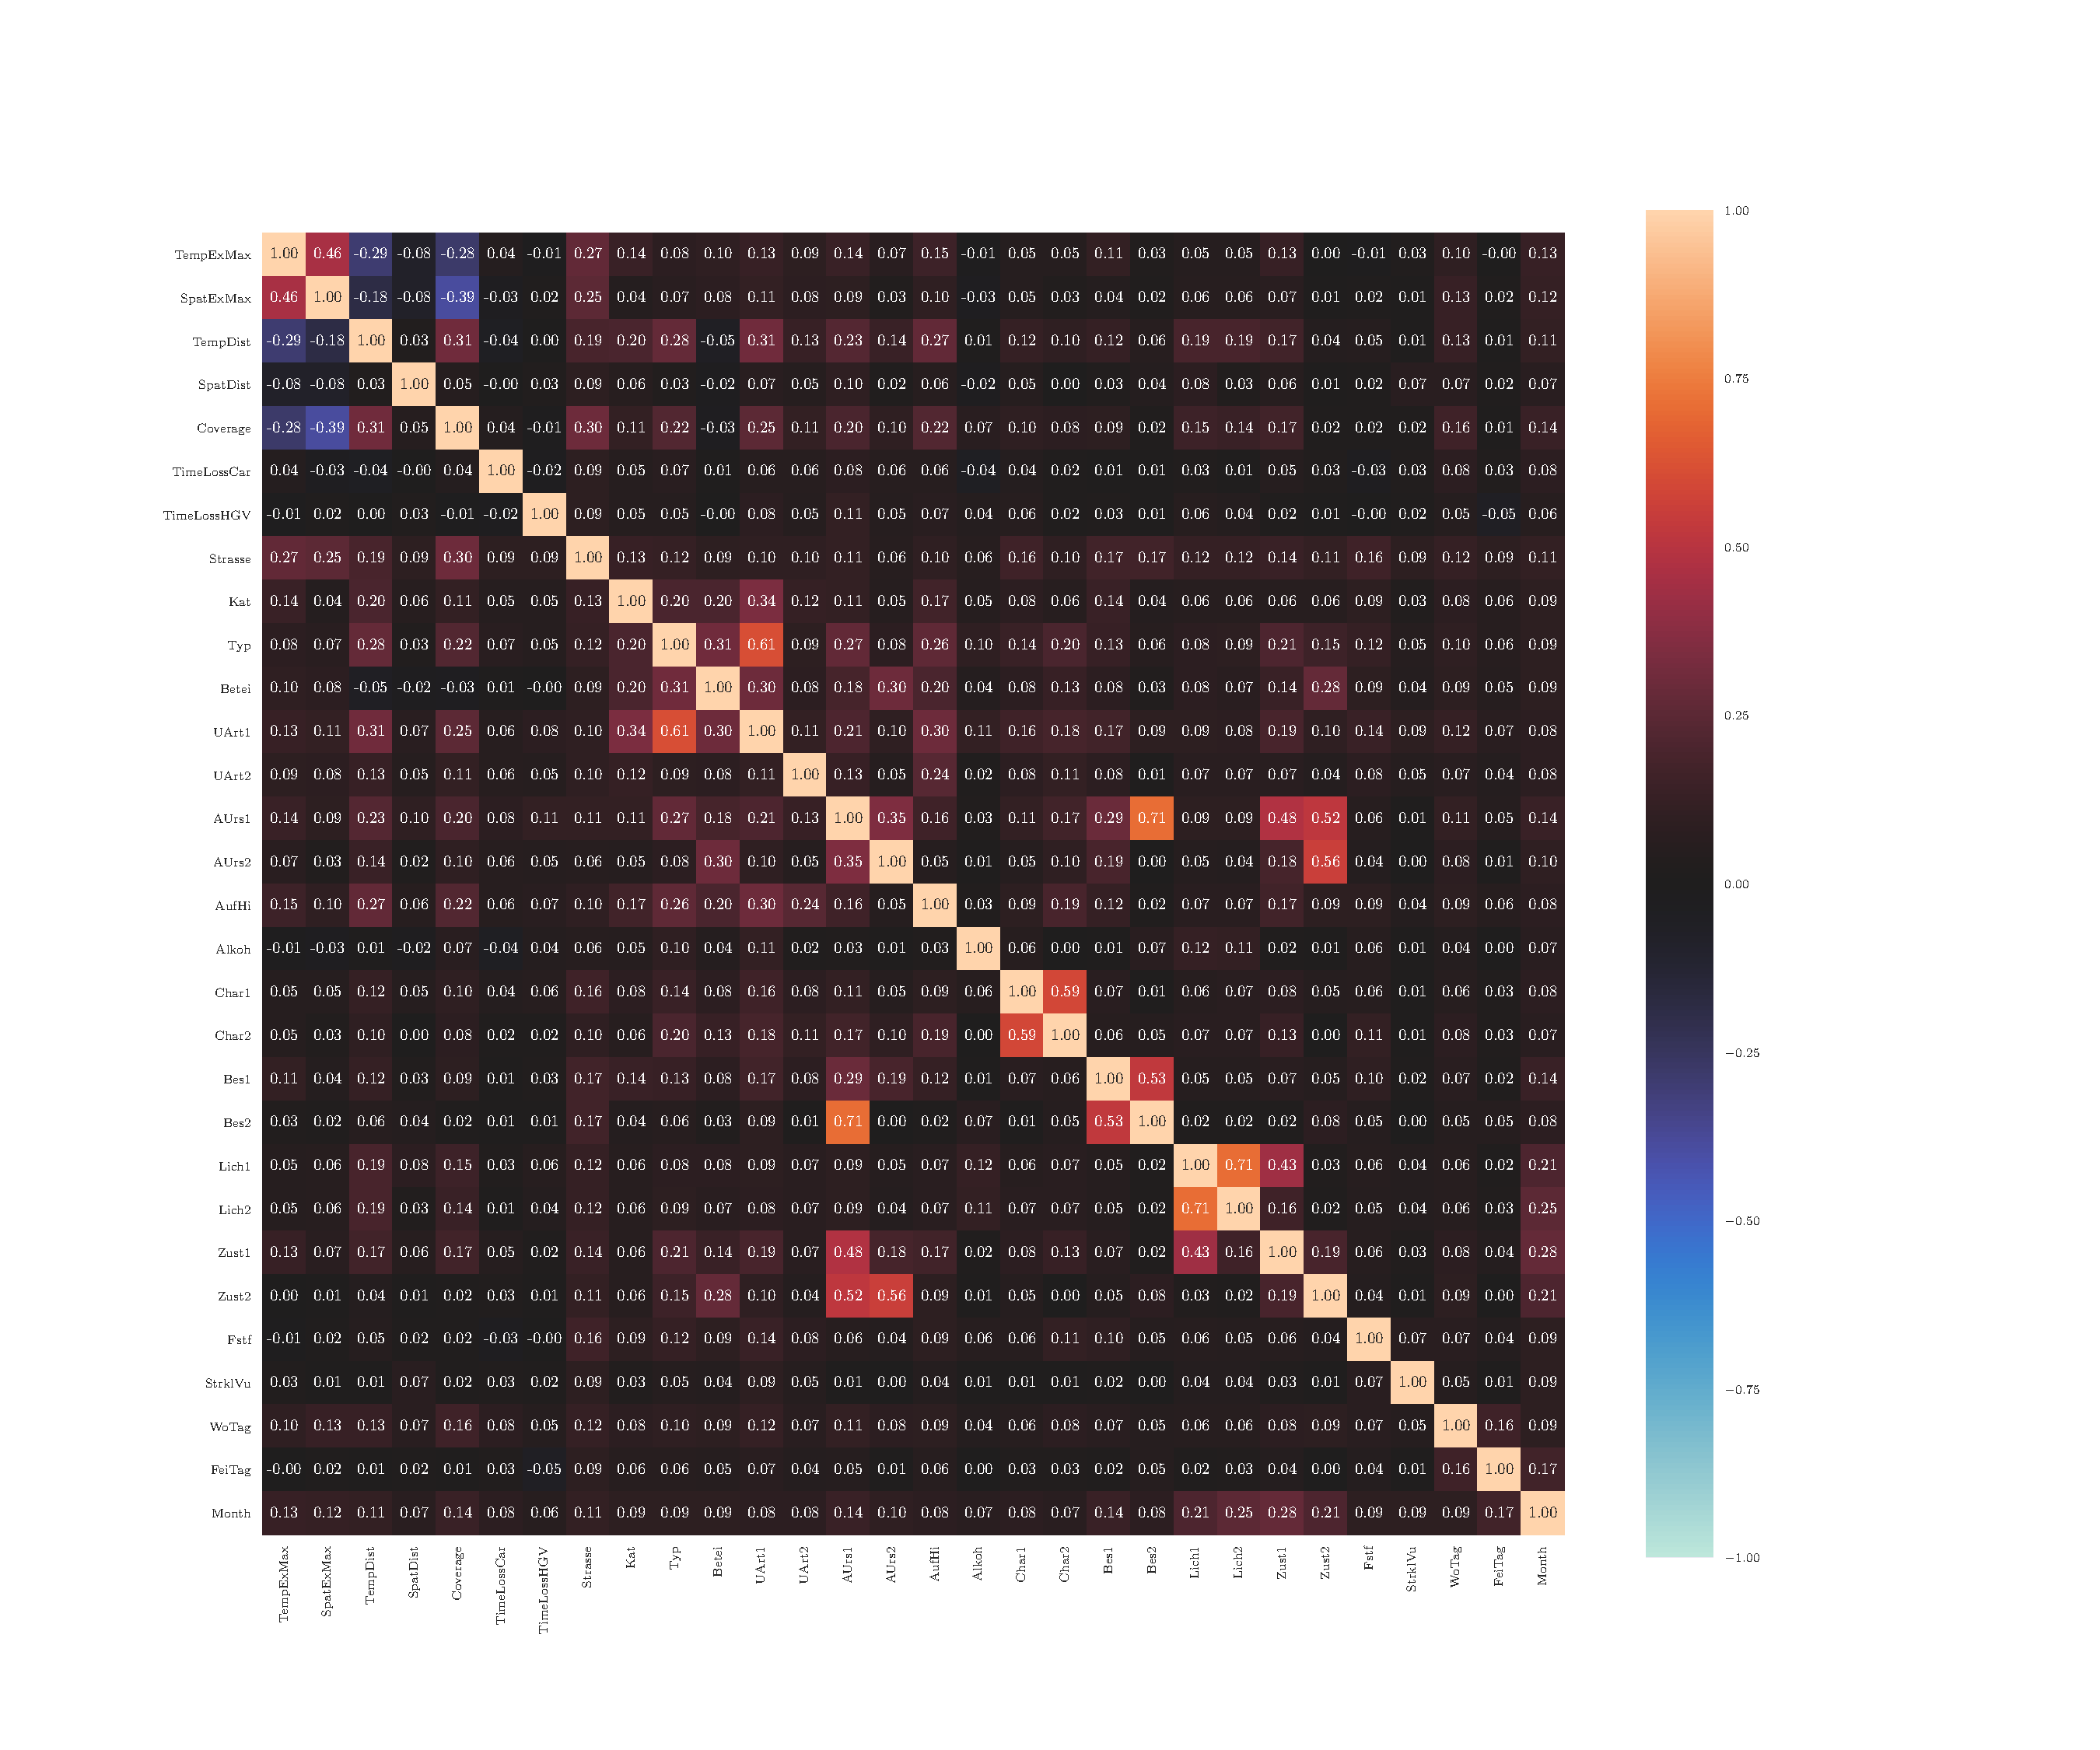
\includegraphics[scale=0.52, trim=3cm 2cm 0cm 0cm]{../CorrAnalysis/data/BAYSIS/02_matched/plots/baysis_matched_corr_cramers}
% 		\caption{Correlation matrix for BAYSIS matched data, with $V$, $\eta$, $\tau$, $r_{pq}$, $r$}
% 		\label{img:correlation_matrix_matched_cramers}
% 	\end{figure}
% \restoregeometry
\begin{figure}[!ht]
	\centering
	\makebox[\textwidth][c]{%
		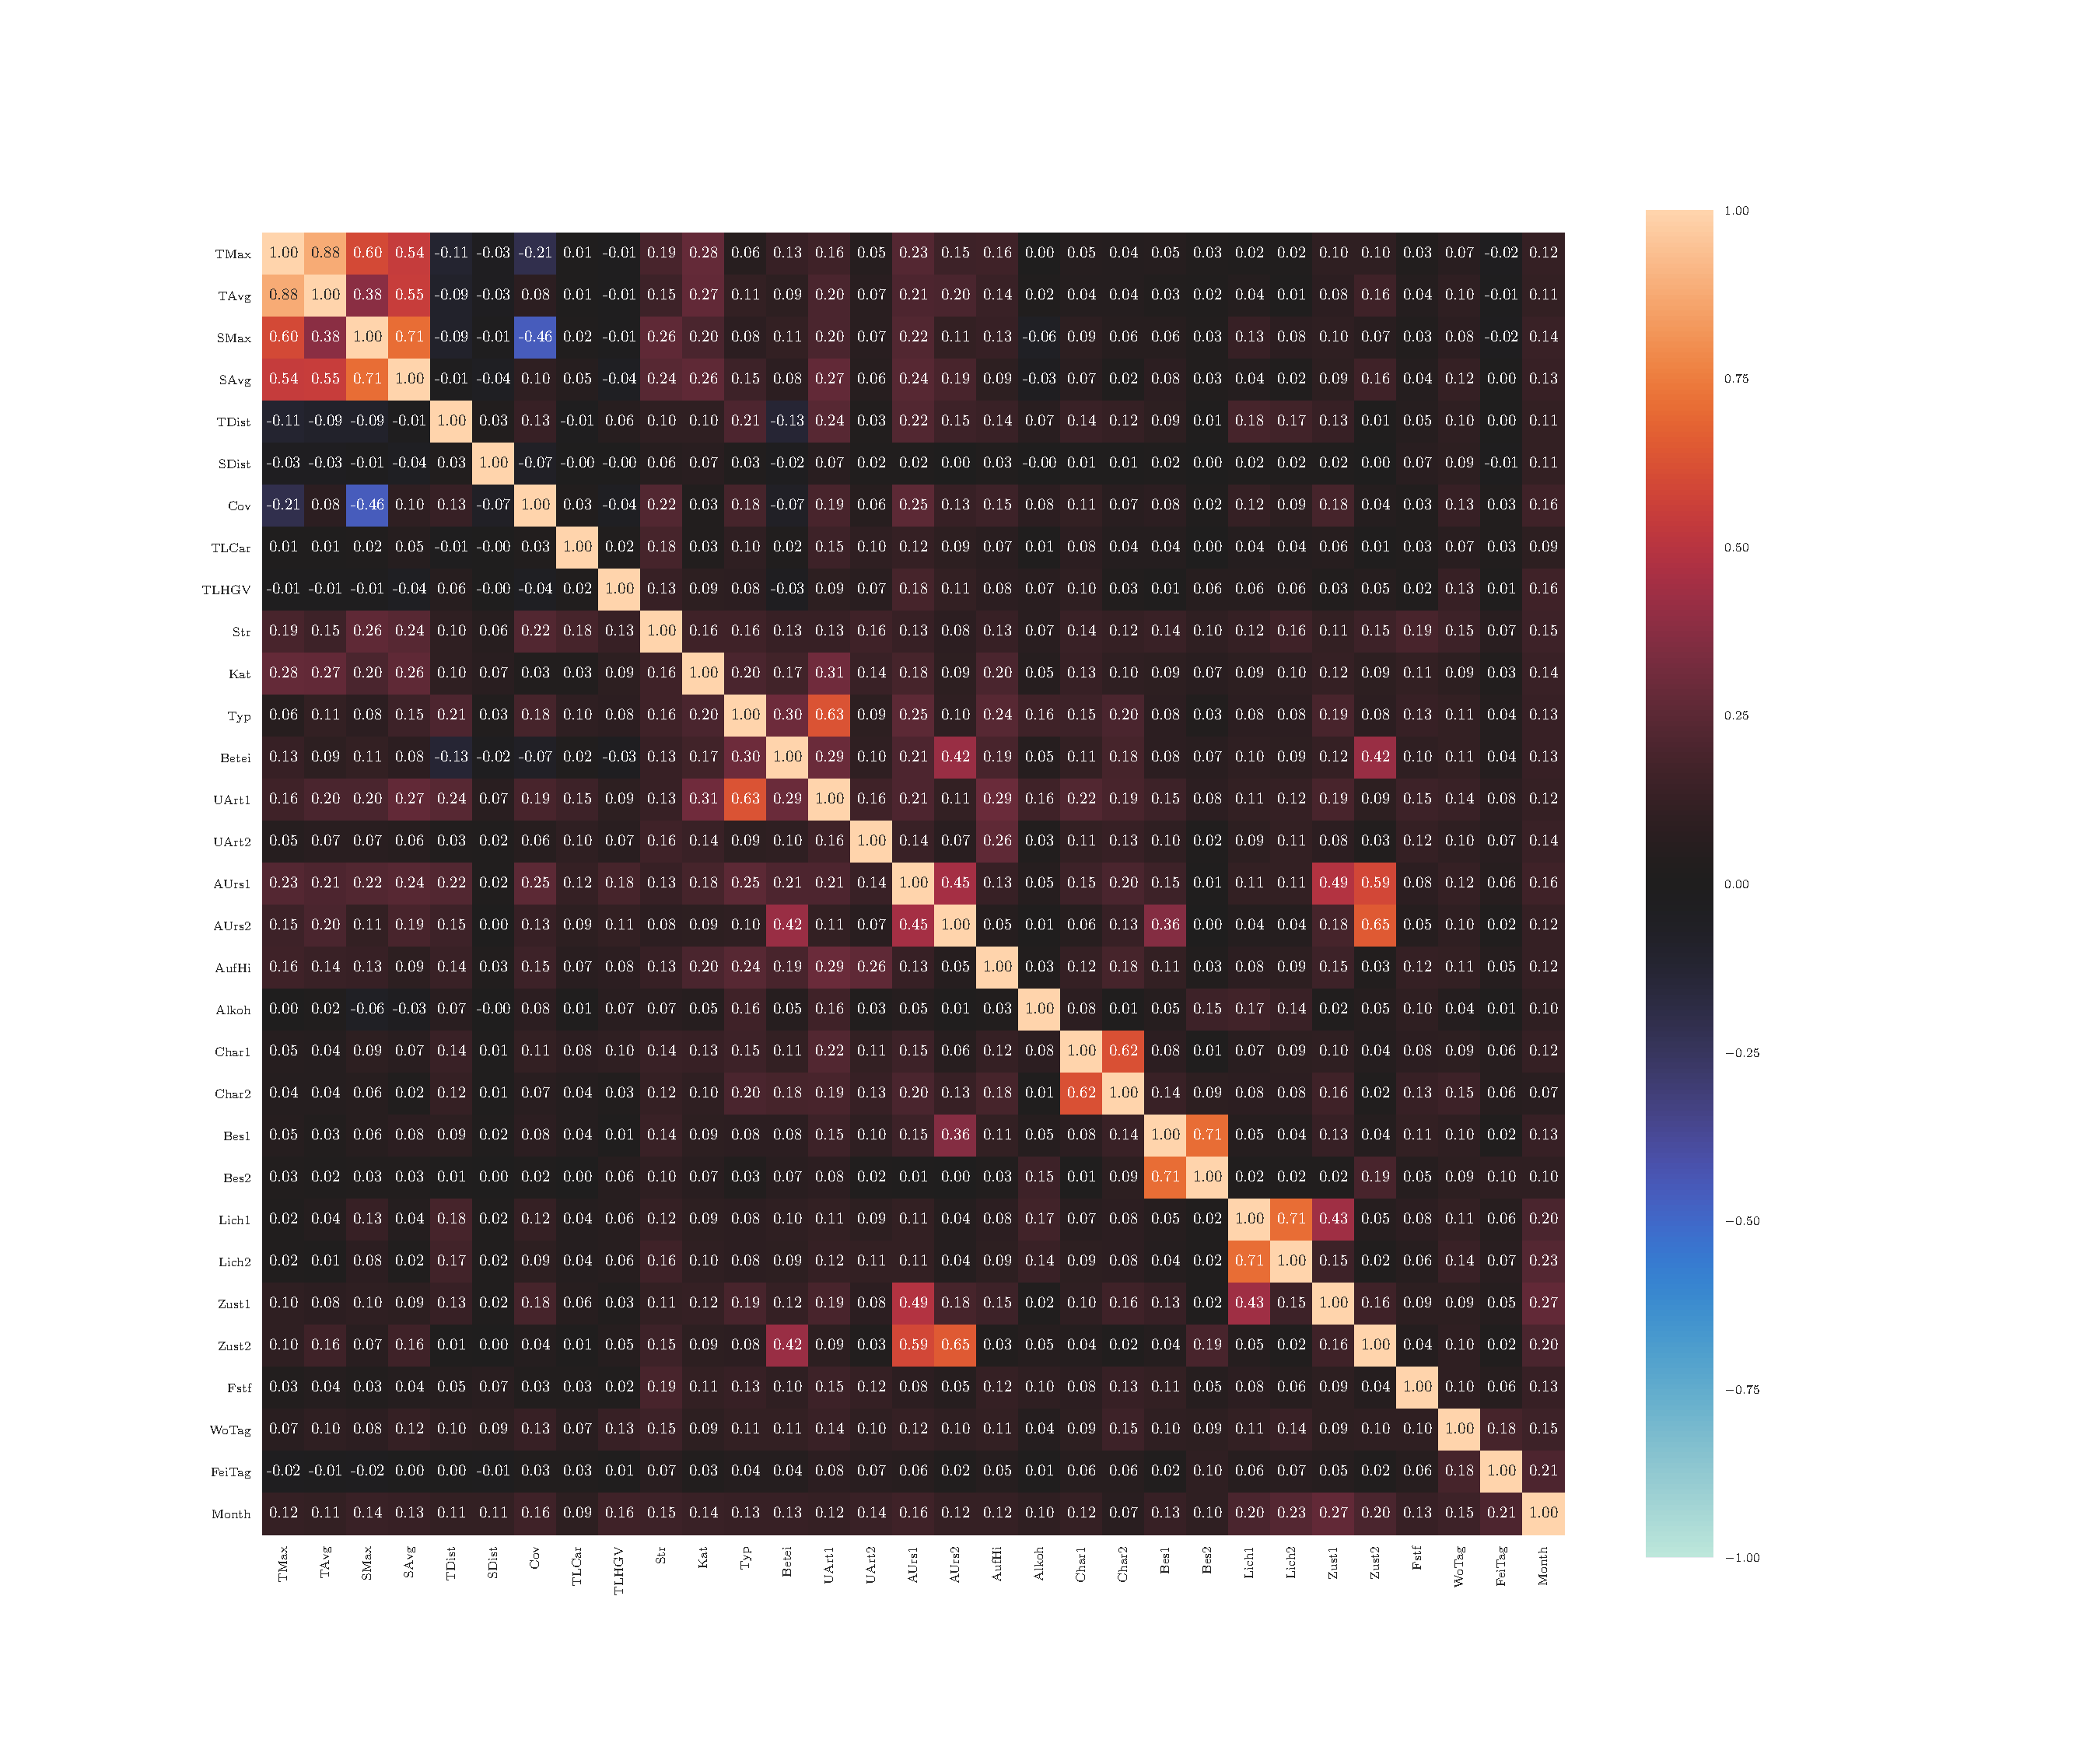
\includegraphics[width=1.4\textwidth, trim=0cm 2.5cm 6cm 3cm]{CorrAnalysis/data/BAYSIS/03_selected_01_startJam/plots/baysis_selected_corr_cramers}%
	}
	\caption{Correlation matrix for congestion-accident matched data classified as \textit{Jam Initiator}, with $V$, $\eta$, $\tau$, $r_{pq}$, $r$}
	\label{img:correlation_matrix_matched_cramers}
\end{figure}

% --------------------------
% -------- Strasse ---------
% --------------------------
\Large
\centerline{\textbf{Strasse}}
\normalsize

\paragraph{Maximal Temporal Extent}
% chi-squared = 151.97, df = 131
The Kruskal-Wallis rank sum test of \textbf{Strasse}-\textbf{TMax} produces a $p$-value of 0.1015, which is above $\alpha=.05$. The null hypothesis can't be rejected and there is \textbf{no} significant difference between the groups of \textbf{Strasse}. There are no significant groups to identify.

\paragraph{Average Temporal Extent}
% chi-squared = 173.3, df = 175
The Kruskal-Wallis rank sum test of \textbf{Strasse}-\textbf{TAvg} produces a $p$-value of 0.5221, which is above $\alpha=.05$. The null hypothesis can't be rejected and there is \textbf{no} significant difference between the groups of \textbf{Strasse}. There are no significant groups to identify.

\paragraph{Maximal Spatial Extent}
% chi-squared = 752.87, df = 720
The Kruskal-Wallis rank sum test of \textbf{Strasse}-\textbf{SMax} produces a $p$-value of 0.1919, which is above $\alpha=.05$. The null hypothesis can't be rejected and there is \textbf{no} significant difference between the groups of \textbf{Strasse}. There are no significant groups to identify.

\paragraph{Average Spatial Extent}
% chi-squared = 753.78, df = 727
The Kruskal-Wallis rank sum test of \textbf{Strasse}-\textbf{SAvg} produces a $p$-value of 0.2385, which is above $\alpha=.05$. The null hypothesis can't be rejected and there is \textbf{no} significant difference between the groups of \textbf{Strasse}. There are no significant groups to identify.

\paragraph{Coverage}
% chi-squared = 112, df = 93
The Kruskal-Wallis rank sum test of \textbf{Strasse}-\textbf{Cov} produces a $p$-value of 0.0875, which is above $\alpha=.05$. The null hypothesis can't be rejected and there is \textbf{no} significant difference between the groups of \textbf{Strasse}. There are no significant groups to identify.

\paragraph{Time-loss Car}
% chi-squared = 547.62, df = 529
The Kruskal-Wallis rank sum test of \textbf{Strasse}-\textbf{TLCar} produces a $p$-value of 0.2788, which is above $\alpha=.05$. The null hypothesis can't be rejected and there is \textbf{no} significant difference between the groups of \textbf{Strasse}. There are no significant groups to identify.

% ----------------------
% -------- Kat ---------
% ----------------------
\Large
\centerline{\textbf{Kat}}
\normalsize
This section analyzes the correlated relations of the variable \textbf{Kat} and introduces a initial interpretation of each significant correlation. Groups with an insufficient sample size (see \cref{correlation_uncertainty} are neglected and not considered. The encoding and description of the variable \textbf{Typ} is shown in \cref{tbl:baysis_dataset_Typ}.
% \begin{table}[!ht]
% 	\centering
% 	\tiny
% 	\begin{tabular}{c|l} 
% 		\toprule
% 		Code & Description \\ 
% 		\midrule
%  		0 	& Minor Accident  \\
%  		1 	& Accident with deaths  \\ 
%  		2 	& Accident with heavily injured  \\
%  		3 	& Accident with lightly injured  \\
% 		7 	& Accident with property damage  \\
% 		\bottomrule
% 	\end{tabular}
% 	\caption{Encoding of \textbf{Kat}}
% 	\label{table:analysis_encoding_Kat}
% 	%\vspace{-8mm}
% \end{table}

\paragraph{Maximal Temporal Extent}
% chi-squared = 196.02, df = 131
The Kruskal-Wallis rank sum test of \textbf{Kat}-\textbf{TMax} produces a $p$-value of 0.0002, which is below $\alpha=.05$. The null hypothesis can therefore be rejected, which means there is a significant difference between the groups of \textbf{Kat}. To identify the significant groups, a pairwise Wilcoxon $T$-test for \textbf{Kat}-\textbf{TMax} is run, which produces \cref{tbl:wilcoxon_baysis_initiator_Kat_TMax}. 
\begin{table}[ht]
	\centering
	\begin{tabular}{rrrr}
		\toprule  
  		& 1 & 2 & 3 \\ 
  		\midrule    
        2 & 0.00 &  &  \\ 
        3 & 0.00 & 0.00 &  \\ 
        7 & 0.00 & 0.00 & 0.00 \\ 
 		\bottomrule
	\end{tabular}
    \caption{Pairwise Wilcoxon $T$-test for \textit{Kat} and \textit{Maximal Temporal Extent}}
    \label{tbl:wilcoxon_baysis_initiator_Kat_TMax}
\end{table}
The matrix shows that there is a general trend and all groups differ significantly. With the descriptives from \cref{tbl:descriptives_baysis_initiator_Kat_TMax} that the $\bar{x}$ and $\tilde{x}$ increases from group 7 to 1. We can therefore interpret that the maximal duration of jams, created by accidents increases with the gravity of the accident.
\begin{table}[ht]
	\centering
	\begin{tabular}{c|c|c|c|c|c|c|c}
		\toprule  
		Group & $n$ & $\bar{x}$ & $\sigma$ & $\tilde{x}$ & $min$ & $max$ & $\Delta$ \\
        \midrule
        1 & 29  & 290.07 & 190.59 & 255.00 & 27 & 864  & 837 \\ 
        2 & 144 & 156.23 & 119.44 & 120.00 & 9  & 657  & 648 \\ 
        3 & 423 & 121.05 & 105.34 & 99.00  & 9  & 1116 & 1107 \\ 
        7 & 181 & 103.13 & 143.89 & 75.00  & 9  & 1341 & 1332 \\ 
 		\bottomrule
	\end{tabular}
    \caption{Descriptives of the groups of \textit{Kat} and \textit{Maximal Temporal Extent}}
    \label{tbl:descriptives_baysis_initiator_Kat_TMax}
\end{table}

\paragraph{Average temporal Extent}
% chi-squared = 222.52, df = 175
The Kruskal-Wallis rank sum test of \textbf{Kat}-\textbf{TAvg} produces a $p$-value of 0.0087, which is way below $\alpha=.05$. The null hypothesis can therefore be rejected, which means there is a significant difference between the groups of \textbf{Kat}. To identify the significant groups, a pairwise Wilcoxon $T$-test for \textbf{Kat}-\textbf{TAvg} is run, which produces \cref{tbl:wilcoxon_baysis_initiator_Kat_TAvg}. 
\begin{table}[ht]
	\small
	\centering
    \begin{tabular}{rrrr}
        \toprule
        & 1 & 2 & 3 \\ 
        \midrule
        2 & 0.00 &  &  \\ 
        3 & 0.00 & 0.01 &  \\ 
        7 & 0.00 & 0.00 & 0.00 \\ 
        \bottomrule
    \end{tabular}
	\caption{Pairwise Wilcoxon $T$-test for \textit{Kat} and \textit{Average Temporal Extent}}
	\label{tbl:wilcoxon_baysis_initiator_Kat_TAvg}
\end{table}
The $p$-values show that all groups differ significantly from each other. The descriptives in table \cref{tbl:descriptives_baysis_initiator_Kat_TAvg}, show that $\bar{x}$ and $\tilde{x}$ increases with the groups from 7 to 1, like \textbf{TAMx}. The interpretation is therefore similar that the average duration of jams created by accident increases with the gravity of the accident.
\begin{table}[ht]
	\small
	\centering
    \begin{tabular}{c|c|c|c|c|c|c|c}
        \toprule
        Group & $n$ & $\bar{x}$ & $\sigma$ & $\tilde{x}$ & $min$ & $max$ & $\Delta$ \\
        \midrule
        1 & 29  & 148.76 & 90.65 & 144.00 & 20 & 376 & 356 \\ 
        2 & 144 & 80.91  & 67.52 & 61.50  & 7  & 426 & 419 \\ 
        3 & 423 & 63.84  & 51.24 & 53.00  & 5  & 469 & 464 \\ 
        7 & 181 & 53.61  & 80.96 & 39.00  & 4  & 920 & 916 \\ 
        \bottomrule
    \end{tabular}
	\caption{Group descriptives of \textit{Kat} and \textit{Average temporal Extent}}
	\label{tbl:descriptives_baysis_initiator_Kat_TAvg}
	%\vspace{-8mm}
\end{table}

\paragraph{Maximal spatial Extent}
% chi-squared = 732.27, df = 720
The Kruskal-Wallis rank sum test of \textbf{Kat}-\textbf{SMax} produces a $p$-value of 0.3673, which is above $\alpha=.05$. The null hypothesis can't be rejected and there is \textbf{no} significant difference between the groups of \textbf{Kat}. There are no significant groups to identify.

\paragraph{Average spatial Extent}
% chi-squared = 738.37, df = 727
The Kruskal-Wallis rank sum test of \textbf{Kat}-\textbf{SAvg} produces a $p$-value of 0.3767, which is above $\alpha=.05$. The null hypothesis can't be rejected and there is \textbf{no} significant difference between the groups of \textbf{Kat}. There are no significant groups to identify.

% ----------------------
% -------- Typ ---------
% ----------------------
\Large
\centerline{\textbf{Typ}}
\normalsize
This section analyzes the correlated relations of the accident variable \textbf{Typ} and introduces a initial interpretation of each significant correlation. Groups with an insufficient sample size (see \cref{correlation_uncertainty} are neglected and not considered. The encoding and description of the variable \textbf{Typ} is shown in \cref{tbl:baysis_dataset_Typ}.
% \begin{table}[ht]
% 	\centering
% 	\tiny
% 	\begin{tabular}{c|l} 
% 		\toprule
% 		Code & Description \\ 
% 		\midrule
%  		1 & Driving accident \\ 
%  		2 & Turning accident \\
%  		3 & Merging / Crossing accident \\
%  		4 & Crossing over accident \\
%  		5 & Accident in standing traffic \\
%  		6 & Accident in straight traffic \\
% 		7 & Other \\
% 		\bottomrule
% 	\end{tabular}
% 	\caption{Encoding of \textbf{Typ}}
% 	\label{table:analysis_encoding_Kat}
% 	%\vspace{-8mm}
% \end{table}

\paragraph{Average spatial Extent}
% chi-squared = 739.95, df = 727
The Kruskal-Wallis rank sum test of \textbf{Kat}-\textbf{SAvg} produces a $p$-value of 0.3613, which is above $\alpha=.05$. The null hypothesis can't be rejected and there is \textbf{no} significant difference between the groups of \textbf{Kat}. There are no significant groups to identify.

\paragraph{Temporal Distance}
% chi-squared = 39.181, df = 24
The Kruskal-Wallis rank sum test of \textbf{Kat}-\textbf{TDist} produces a $p$-value of 0.0261, which is way below $\alpha=.05$. The null hypothesis can therefore be rejected, which means there is a significant difference between the groups of \textbf{Kat}. To identify the significant groups, a pairwise Wilcoxon $T$-test for \textbf{Kat}-\textbf{TDist} is run, which produces \cref{tbl:wilcoxon_baysis_initiator_Typ_TDist}. 
\begin{table}[ht]
	\small
	\centering
    \begin{tabular}{rrrrrr}
        \toprule
        & 1 & 3 & 4 & 5 & 6 \\ 
        \midrule
        3 & 0.05 &  &  &  &  \\ 
        4 & 1.00 & 0.38 &  &  &  \\ 
        5 & 0.96 & 1.00 & 0.96 &  &  \\ 
        6 & 0.00 & 0.96 & 0.51 & 1.00 &  \\ 
        7 & 1.00 & 0.04 & 1.00 & 0.96 & 0.01 \\ 
        \bottomrule
    \end{tabular}
    \caption{Pairwise Wilcoxon $T$-test for \textit{Typ} and \textit{Temporal Distance}}
    \label{tbl:wilcoxon_baysis_initiator_Typ_TDist}
\end{table}
The significance matrix \cref{tbl:wilcoxon_baysis_initiator_Typ_TDist} shows that group 6 differs from group 1 and group 7 differs from 6. The descriptives from \cref{tbl:descriptives_baysis_initiator_Typ_TDist} also shows that the temporal distance in group 1 and 7 is 25\,\% higher than in group 6. Group 3 also shows a substantial gap in $\bar{x}$
but only is barely significance with $p=.05$. Because the groups of $driving$ and $straight traffic$ accidents are very similar, there is no clear interpretation to be drawn.
\begin{table}[ht]
	\small
	\centering
    \begin{tabular}{c|c|c|c|c|c|c|c}
        \toprule
        Group & $n$ & $\bar{x}$ & $\sigma$ & $\tilde{x}$ & $min$ & $max$ & $\Delta$ \\
        \midrule
        1 & 181 & 11.40 & 6.38 & 10.00 & 1  & 24 & 23 \\ 
        3 & 24  & 7.67  & 6.06 & 7.00  & 1  & 22 & 21 \\ 
        %4 & 4   & 14.00 & 3.92 & 13.50 & 10 & 19 & 9 \\ 
        %5 & 2   & 4.50  & 3.54 & 4.50  & 2  & 7  & 5 \\ 
        6 & 496 & 9.20  & 5.88 & 8.00  & 0  & 24 & 24 \\ 
        7 & 70  & 12.27 & 7.09 & 11.00 & 0  & 24 & 24 \\ 
        \bottomrule
    \end{tabular}
    \caption{Group descriptives of \textit{Typ} and \textit{Temporal Distance}}
    \label{tbl:descriptives_baysis_initiator_Typ_TDist}
	%\vspace{-8mm}
\end{table}

\paragraph{Coverage}
% chi-squared = 87.648, df = 93
The Kruskal-Wallis rank sum test of \textbf{Kat}-\textbf{Cov} produces a $p$-value of 0.6372, which is above $\alpha=.05$. The null hypothesis can't be rejected and there is \textbf{no} significant difference between the groups of \textbf{Kat}. There are no significant groups to identify.

% ------------------------
% -------- UArt1 ---------
% ------------------------
\Large
\centerline{\textbf{UArt1}}
\normalsize
This section analyzes the correlated relations of the accident variable \textbf{UArt} and introduces a initial interpretation of each significant correlation. Groups with an insufficient sample size (see \cref{correlation_uncertainty} are neglected and not considered. The encoding and description of the variable \textbf{UArt} is shown in \cref{tbl:baysis_dataset_UArt}. 
% \begin{table}[ht]
% 	\centering
% 	\tiny
% 	\begin{tabular}{c|l} 
% 		\toprule
% 		Code & Description \\ 
% 		\midrule
%  		1 & Collision with starting, standing or stopping vehicle  \\ 
%  		2 & Collision with ahead and waiting vehicle  \\
%  		3 & Collision with vehicle on separate lane in same direction  \\
%  		4 & Collision with vehicle going in opposite direction  \\
%  		5 & Collision with turning or crossing vehicle  \\
%  		6 & Collision between vehicle and pedestrian  \\
%  		7 & Collision with obstacle  \\
%  		8 & Deviation to the right  \\
%  		9 & Deviation to the left  \\
% 		0 & Other  \\
% 		\bottomrule
% 	\end{tabular}
% 	\caption{Descriptive of \textbf{UArt}}
% 	\label{table:analysis_encoding_UArt}
% 	%\vspace{-8mm}
% \end{table}


\paragraph{Maximal Temporal Extent}
% chi-squared = 184.29, df = 131
The Kruskal-Wallis rank sum test of \textbf{UArt}-\textbf{TMax} produces a $p$-value of 0.0015, which is way below $\alpha=.05$. The null hypothesis can therefore be rejected, which means there is a significant difference between the groups of \textbf{UArt}. To identify the significant groups, a pairwise Wilcoxon $T$-test for \textbf{UArt}-\textbf{TMax} is run, which produces \cref{tbl:wilcoxon_baysis_initiator_UArt_TMax}. 
\begin{table}[ht]
	\small
	\centering
    \begin{tabular}{rrrrrrrrrr}
        \toprule
        & 0 & 1 & 2 & 3 & 4 & 5 & 6 & 7 & 8 \\ 
        \midrule
        1 & 1.00 &  &  &  &  &  &  &  &  \\ 
        2 & 1.00 & 1.00 &  &  &  &  &  &  &  \\ 
        3 & 1.00 & 0.04 & 0.00 &  &  &  &  &  &  \\ 
        4 & 1.00 & 1.00 & 1.00 & 1.00 &  &  &  &  &  \\ 
        5 & 1.00 & 1.00 & 1.00 & 1.00 & 1.00 &  &  &  &  \\ 
        6 & 1.00 & 1.00 & 1.00 & 1.00 & 1.00 & 1.00 &  &  &  \\ 
        7 & 0.75 & 0.05 & 0.12 & 1.00 & 1.00 & 1.00 & 1.00 &  &  \\ 
        8 & 1.00 & 0.21 & 0.43 & 1.00 & 1.00 & 1.00 & 1.00 & 1.00 &  \\ 
        9 & 1.00 & 0.43 & 1.00 & 1.00 & 1.00 & 1.00 & 1.00 & 1.00 & 1.00 \\ 
        \bottomrule
      \end{tabular}
    \caption{Pairwise Wilcoxon $T$-test for \textit{UArt} and \textit{Maximal Temporal Extent}}
    \label{tbl:wilcoxon_baysis_initiator_UArt_TMax}
\end{table}
\todo{Explain}
\begin{table}[ht]
	\small
	\centering
    \begin{tabular}{c|c|c|c|c|c|c|c}
        \toprule
        Group & $n$ & $\bar{x}$ & $\sigma$ & $\tilde{x}$ & $min$ & $max$ & $\Delta$ \\
        \midrule
        0 & 24  & 140.75 & 100.75 & 114.00 & 30 & 375  & 345 \\ 
        1 & 31  & 198.58 & 166.25 & 126.00 & 39 & 612  & 573 \\ 
        2 & 345 & 134.87 & 108.69 & 105.00 & 9  & 864  & 855  \\ 
        3 & 144 & 111.79 & 123.13 & 81.00  & 9  & 1116 & 1107 \\ 
        4 & 4   & 186.00 & 145.68 & 175.50 & 39 & 354  & 315 \\ 
        5 & 15  & 179.60 & 324.31 & 99.00  & 15 & 1341 & 1326 \\ 
        6 & 4   & 171.00 & 98.62  & 178.50 & 66 & 261  & 195 \\ 
        7 & 23  & 87.91  & 93.15  & 48.00  & 12 & 384  & 372 \\ 
        8 & 107 & 118.46 & 117.62 & 87.00  & 18 & 813  & 795 \\ 
        9 & 80  & 122.47 & 143.91 & 91.50  & 12 & 1152 & 1140 \\ 
        \bottomrule
      \end{tabular}
    \caption{Group descriptives of \textit{UArt} and \textit{Maximal Temporal Extent}}
    \label{tbl:descriptives_baysis_initiator_UArt_TMax}
	%\vspace{-8mm}
\end{table}

\paragraph{Average Temporal Extent}
% chi-squared = 182.51, df = 175
The Kruskal-Wallis rank sum test of \textbf{UArt}-\textbf{TAvg} produces a $p$-value of 0.3331, which is above $\alpha=.05$. The null hypothesis can't be rejected and there is \textbf{no} significant difference between the groups of \textbf{UArt}. There are no significant groups to identify.

\paragraph{Maximal Spatial Extent}
% chi-squared = 735.57, df = 720
The Kruskal-Wallis rank sum test of \textbf{UArt}-\textbf{SMax} produces a $p$-value of 0.3355, which is above $\alpha=.05$. The null hypothesis can't be rejected and there is \textbf{no} significant difference between the groups of \textbf{UArt}. There are no significant groups to identify.

\paragraph{Average Spatial Extent}
% chi-squared = 741.73, df = 727
The Kruskal-Wallis rank sum test of \textbf{UArt}-\textbf{SAvg} produces a $p$-value of 0.3442, which is above $\alpha=.05$. The null hypothesis can't be rejected and there is \textbf{no} significant difference between the groups of \textbf{UArt}. There are no significant groups to identify.

\paragraph{Temporal Distance}
% chi-squared = 43.627, df = 24
The Kruskal-Wallis rank sum test of \textbf{UArt}-\textbf{TDist} produces a $p$-value of 0.0084, which is way below $\alpha=.05$. The null hypothesis can therefore be rejected, which means there is a significant difference between the groups of \textbf{UArt}. To identify the significant groups, a pairwise Wilcoxon $T$-test for \textbf{UArt}-\textbf{TDist} is run, which produces \cref{tbl:wilcoxon_baysis_initiator_UArt_TDist}. 
\begin{table}[ht]
	\small
	\centering
    \begin{tabular}{rrrrrrrrrr}
        \toprule
        & 0 & 1 & 2 & 3 & 4 & 5 & 6 & 7 & 8 \\ 
        \midrule
        1 & 1.00 &  &  &  &  &  &  &  &  \\ 
        2 & 1.00 & 1.00 &  &  &  &  &  &  &  \\ 
        3 & 1.00 & 1.00 & 1.00 &  &  &  &  &  &  \\ 
        4 & 1.00 & 1.00 & 1.00 & 1.00 &  &  &  &  &  \\ 
        5 & 1.00 & 1.00 & 1.00 & 1.00 & 1.00 &  &  &  &  \\ 
        6 & 1.00 & 1.00 & 1.00 & 1.00 & 1.00 & 1.00 &  &  &  \\ 
        7 & 1.00 & 0.06 & 0.00 & 0.00 & 1.00 & 0.10 & 1.00 &  &  \\ 
        8 & 1.00 & 1.00 & 0.01 & 0.01 & 1.00 & 1.00 & 1.00 & 1.00 &  \\ 
        9 & 1.00 & 1.00 & 0.05 & 0.01 & 1.00 & 0.78 & 1.00 & 0.87 & 1.00 \\ 
        \bottomrule
      \end{tabular}
    \caption{Pairwise Wilcoxon $T$-test for \textit{UArt} and \textit{Temporal Distance}}
    \label{tbl:wilcoxon_baysis_initiator_UArt_TDist}
\end{table}
\todo{Explain}
\begin{table}[ht]
	\small
	\centering
    \begin{tabular}{c|c|c|c|c|c|c|c}
        \toprule
        Group & $n$ & $\bar{x}$ & $\sigma$ & $\tilde{x}$ & $min$ & $max$ & $\Delta$ \\
        \midrule
        0 & 24  & 11.04 & 6.22 & 10.00 & 2  & 22 & 20 \\ 
        1 & 31  & 8.94  & 6.03 & 7.00  & 0  & 24 & 24 \\ 
        2 & 345 & 9.21  & 5.90 & 8.00  & 1  & 24 & 23 \\ 
        3 & 144 & 8.80  & 6.03 & 7.00  & 1  & 24 & 23 \\ 
        4 & 4   & 12.00 & 4.08 & 10.50 & 9  & 18 & 9  \\ 
        5 & 15  & 8.13  & 7.06 & 7.00  & 0  & 22 & 22 \\ 
        6 & 4   & 14.00 & 3.92 & 13.50 & 10 & 19 & 9  \\ 
        7 & 23  & 15.26 & 7.04 & 14.00 & 4  & 24 & 20 \\ 
        8 & 107 & 11.81 & 6.57 & 11.00 & 1  & 24 & 23 \\ 
        9 & 80  & 11.38 & 5.87 & 10.00 & 2  & 24 & 22 \\ 
        \bottomrule
      \end{tabular}
    \caption{Group descriptives of \textit{UArt} and \textit{Temporal Distance}}
    \label{tbl:descriptives_baysis_initiator_UArt_TDist}
	%\vspace{-8mm}
\end{table}

\paragraph{Coverage}
% chi-squared = 119.45, df = 93
The Kruskal-Wallis rank sum test of \textbf{UArt}-\textbf{Cov} produces a $p$-value of 0.0337, which is way below $\alpha=.05$. The null hypothesis can therefore be rejected, which means there is a significant difference between the groups of \textbf{UArt}. To identify the significant groups, a pairwise Wilcoxon $T$-test for \textbf{UArt}-\textbf{Cov} is run, which produces \cref{tbl:wilcoxon_baysis_initiator_UArt_TDist}. 
\begin{table}[ht]
	\small
	\centering
    \begin{tabular}{rrrrrrrrrr}
        \toprule
        & 0 & 1 & 2 & 3 & 4 & 5 & 6 & 7 & 8 \\ 
        \midrule
        1 & 1.00 &  &  &  &  &  &  &  &  \\ 
        2 & 1.00 & 1.00 &  &  &  &  &  &  &  \\ 
        3 & 1.00 & 1.00 & 1.00 &  &  &  &  &  &  \\ 
        4 & 1.00 & 1.00 & 1.00 & 1.00 &  &  &  &  &  \\ 
        5 & 1.00 & 1.00 & 1.00 & 1.00 & 1.00 &  &  &  &  \\ 
        6 & 1.00 & 1.00 & 1.00 & 1.00 & 1.00 & 1.00 &  &  &  \\ 
        7 & 1.00 & 1.00 & 1.00 & 1.00 & 1.00 & 1.00 & 1.00 &  &  \\ 
        8 & 1.00 & 1.00 & 0.12 & 0.09 & 1.00 & 0.72 & 1.00 & 1.00 &  \\ 
        9 & 1.00 & 1.00 & 1.00 & 1.00 & 1.00 & 1.00 & 1.00 & 1.00 & 1.00 \\ 
        \bottomrule
      \end{tabular}
    \caption{Pairwise Wilcoxon $T$-test for \textit{UArt} and \textit{Coverage}}
    \label{tbl:wilcoxon_baysis_initiator_UArt_Cov}
\end{table}
\todo{Explain}
\begin{table}[ht]
	\small
	\centering
    \begin{tabular}{c|c|c|c|c|c|c|c}
        \toprule
        Group & $n$ & $\bar{x}$ & $\sigma$ & $\tilde{x}$ & $min$ & $max$ & $\Delta$ \\
        \midrule
        0 & 24  & 51.38 & 20.70 & 45.50 & 23 & 96  & 73 \\ 
        1 & 31  & 53.68 & 18.85 & 50.00 & 28 & 96  & 68 \\ 
        2 & 345 & 50.71 & 19.95 & 50.00 & 7  & 100 & 93 \\ 
        3 & 144 & 48.90 & 19.87 & 50.00 & 5  & 98  & 93 \\ 
        4 & 4   & 58.00 & 21.10 & 59.00 & 36 & 78  & 42 \\ 
        5 & 15  & 43.27 & 21.32 & 42.00 & 12 & 88  & 76 \\ 
        6 & 4   & 74.75 & 18.93 & 80.50 & 48 & 90  & 42 \\ 
        7 & 23  & 59.09 & 25.74 & 62.00 & 18 & 100 & 82 \\ 
        8 & 107 & 58.85 & 23.92 & 57.00 & 7  & 100 & 93 \\ 
        9 & 80  & 56.73 & 21.86 & 54.00 & 18 & 100 & 82 \\ 
        \bottomrule
      \end{tabular}
    \caption{Group descriptives of \textit{UArt} and \textit{Coverage}}
    \label{tbl:descriptives_baysis_initiator_UArt_Cov}
	%\vspace{-8mm}
\end{table}

\paragraph{Time-Loss Car}
% chi-squared = 525, df = 529
The Kruskal-Wallis rank sum test of \textbf{UArt}-\textbf{TLCar} produces a $p$-value of 0.5409, which is above $\alpha=.05$. The null hypothesis can't be rejected and there is \textbf{no} significant difference between the groups of \textbf{UArt}. There are no significant groups to identify.

% ------------------------
% -------- AUrs1 ---------
% ------------------------
\Large
\centerline{\textbf{AUrs1}}
\normalsize
This section analyzes the correlated relations of the accident variable \textbf{AUrs} and introduces a initial interpretation of each significant correlation. Groups with an insufficient sample size (see \cref{correlation_uncertainty} are neglected and not considered. The encoding and description of the variable \textbf{AUrs} is shown in \cref{tbl:baysis_dataset_AUrs}. The variable value of group 0, which occurs in the dataset is undefined by BAYSIS and will be therefore neglected for the interpretation.
% \begin{table}[ht]
% 	\centering
% 	\small
% 	\begin{tabular}{c|l}
% 		\toprule
% 		Code & Description \\ 
% 		\midrule
% 		70 & Slippery street due to oil \\
% 		71 & Slippery street due to dirt \\
% 		72 & Slippery street due to snow or ice \\
% 		73 & Slippery street due to rain \\
% 		74 & Slippery street due to other objects \\
% 		75 & Cart track due to rain, snow or ice \\
% 		76 & Other condition of road \\
% 		77 & Un-regular condition of traffic signs \\
% 		78 & Bad lighting of street \\
% 		79 & Bad safety on train crossing \\
% 		80 & Visibility issues due to fog \\
% 		81 & Visibility issues due to rain or hail \\
% 		82 & Visibility issues due to sun or glare \\
% 		83 & Crosswind \\
% 		84 & Visibility issues due to storm \\
% 		85 & Unsafe roadwork \\
% 		86 & Wild animals \\
% 		87 & Other animals \\
% 		88 & Other obstacles \\
% 		89 & Other causes \\
% 		% Count[1] 0 = 8435 / Count[2] 0 = 10156
% 		\bottomrule
% 	\end{tabular}
% 	\caption{Descriptive of \textbf{AUrs}}
% 	\label{table:analysis_encoding_AUrs}
% 	\vspace{-8mm}
% \end{table}

\paragraph{Maximal Temporal Extent}
% chi-squared = 136.52, df = 131
The Kruskal-Wallis rank sum test of \textbf{AUrs1}-\textbf{TMax} produces a $p$-value of 0.3529, which is above $\alpha=.05$. The null hypothesis can't be rejected and there is \textbf{no} significant difference between the groups of \textbf{AUrs1}. There are no significant groups to identify.
\paragraph{Average Temporal Extent}
% chi-squared = 205.3, df = 175
The Kruskal-Wallis rank sum test of \textbf{AUrs1}-\textbf{TMax} produces a $p$-value of 0.05823, which is above $\alpha=.05$. The null hypothesis can't be rejected and there is \textbf{no} significant difference between the groups of \textbf{AUrs1}. There are no significant groups to identify.
\paragraph{Maximal Spatial Extent}
% chi-squared = 746.53, df = 720
The Kruskal-Wallis rank sum test of \textbf{AUrs1}-\textbf{TMax} produces a $p$-value of 0.2394, which is above $\alpha=.05$. The null hypothesis can't be rejected and there is \textbf{no} significant difference between the groups of \textbf{AUrs1}. There are no significant groups to identify.
\paragraph{Average Spatial Extent}
% chi-squared = 734.88, df = 727
The Kruskal-Wallis rank sum test of \textbf{AUrs1}-\textbf{TMax} produces a $p$-value of 0.4117, which is above $\alpha=.05$. The null hypothesis can't be rejected and there is \textbf{no} significant difference between the groups of \textbf{AUrs1}. There are no significant groups to identify.
\paragraph{Temporal Distance}
% chi-squared = 31.402, df = 24
The Kruskal-Wallis rank sum test of \textbf{AUrs1}-\textbf{TMax} produces a $p$-value of 0.1425, which is above $\alpha=.05$. The null hypothesis can't be rejected and there is \textbf{no} significant difference between the groups of \textbf{AUrs1}. There are no significant groups to identify.
\paragraph{Coverage}
% chi-squared = 123.97, df = 93
The Kruskal-Wallis rank sum test of \textbf{AUrs1}-\textbf{Cov} produces a $p$-value of 0.0176, which is way below $\alpha=.05$. The null hypothesis can therefore be rejected, which means there is a significant difference between the groups of \textbf{AUrs1}. To identify the significant groups, a pairwise Wilcoxon $T$-test for \textbf{AUrs1}-\textbf{Cov} is run, which produces \cref{tbl:wilcoxon_baysis_initiator_AUrs1_Cov}. 
\begin{table}[ht]
	\small
	\centering
    \begin{tabular}{rrrrrrrrrrrrr}
        \toprule
        & 0 & 72 & 73 & 75 & 77 & 81 & 82 & 83 & 84 & 86 & 87 & 88 \\ 
        \midrule
        72 & 0.01 &  &  &  &  &  &  &  &  &  &  &  \\ 
        73 & 0.24 & 0.63 &  &  &  &  &  &  &  &  &  &  \\ 
        75 & 1.00 & 1.00 & 1.00 &  &  &  &  &  &  &  &  &  \\ 
        77 & 1.00 & 1.00 & 1.00 & 1.00 &  &  &  &  &  &  &  &  \\ 
        81 & 1.00 & 1.00 & 1.00 & 1.00 & 1.00 &  &  &  &  &  &  &  \\ 
        82 & 1.00 & 1.00 & 1.00 & 1.00 & 1.00 & 1.00 &  &  &  &  &  &  \\ 
        83 & 1.00 & 1.00 & 1.00 & 1.00 & 1.00 & 1.00 & 1.00 &  &  &  &  &  \\ 
        84 & 1.00 & 1.00 & 1.00 & 1.00 & 1.00 & 1.00 & 1.00 & 1.00 &  &  &  &  \\ 
        86 & 1.00 & 1.00 & 1.00 & 1.00 & 1.00 & 1.00 & 1.00 & 1.00 & 1.00 &  &  &  \\ 
        87 & 1.00 & 1.00 & 1.00 & 1.00 & 1.00 & 1.00 & 1.00 & 1.00 & 1.00 & 1.00 &  &  \\ 
        88 & 1.00 & 1.00 & 1.00 & 1.00 & 1.00 & 1.00 & 1.00 & 1.00 & 1.00 & 1.00 & 1.00 &  \\ 
        89 & 1.00 & 0.33 & 0.96 & 1.00 & 1.00 & 1.00 & 1.00 & 1.00 & 1.00 & 0.91 & 1.00 & 1.00 \\ 
        \bottomrule
    \end{tabular}
    \caption{Pairwise Wilcoxon $T$-test for \textit{AUrs1} and \textit{Coverage}}
    \label{tbl:wilcoxon_baysis_initiator_AUrs1_Cov}
\end{table}
\todo{Explain}
\begin{table}[ht]
	\small
	\centering
    \begin{tabular}{c|c|c|c|c|c|c|c}
        \toprule
        Group & $n$ & $\bar{x}$ & $\sigma$ & $\tilde{x}$ & $min$ & $max$ & $\Delta$ \\
        \midrule
        0  & 663 & 51.10  & 20.67 & 50.00  & 5   & 100 & 95 \\ 
        72 & 20  & 72.75  & 26.16 & 87.50  & 20  & 100 & 80 \\ 
        73 & 63  & 59.16  & 20.47 & 59.00  & 15  & 100 & 85 \\ 
        %75 & 1   & 100.00 &       & 100.00 & 100 & 100 & 0 \\ 
        %77 & 1   & 79.00  &       & 79.00  & 79  & 79  & 0 \\ 
        %81 & 3   & 61.67  & 26.10 & 59.00  & 37  & 89  & 527 \\ 
        %82 & 5   & 43.20  & 7.22  & 45.00  & 33  & 51  & 18 \\ 
        %83 & 1   & 76.00  &       & 76.00  & 76  & 76  & 0 \\ 
        %84 & 1   & 32.00  &       & 32.00  & 32  & 32  & 0 \\ 
        %86 & 3   & 83.00  & 13.00 & 90.00  & 68  & 91  & 23 \\ 
        %87 & 1   & 67.00  &       & 67.00  & 67  & 67  & 0 \\ 
        %88 & 4   & 66.50  & 26.56 & 71.00  & 35  & 89  & 54 \\ 
        89 & 11  & 43.45  & 11.22 & 42.00  & 25  & 62  & 37 \\ 
        \bottomrule
      \end{tabular}
    \caption{Group descriptives of \textit{AUrs1} and \textit{Coverage}}
    \label{tbl:descriptives_baysis_initiator_AUrs1_Cov}
	%\vspace{-8mm}
\end{table}

\paragraph{Time-loss HGV}
% chi-squared = 416.29, df = 391
The Kruskal-Wallis rank sum test of \textbf{AUrs1}-\textbf{TLHGV} produces a $p$-value of 0.1816, which is above $\alpha=.05$. The null hypothesis can't be rejected and there is \textbf{no} significant difference between the groups of \textbf{AUrs1}. There are no significant groups to identify.

\medskip
Next the second \textbf{AUrs} variable \textbf{AUrs2} will be tested.
\medskip

\paragraph{Maximal Temporal Extent}
% chi-squared = 105.63, df = 131
The Kruskal-Wallis rank sum test of \textbf{AUrs2}-\textbf{TMax} produces a $p$-value of 0.9495, which is above $\alpha=.05$. The null hypothesis can't be rejected and there is \textbf{no} significant difference between the groups of \textbf{AUrs2}. There are no significant groups to identify.

\paragraph{Average Temporal Extent}
% chi-squared = 180.61, df = 175
The Kruskal-Wallis rank sum test of \textbf{AUrs2}-\textbf{TAvg} produces a $p$-value of 0.3698, which is above $\alpha=.05$. The null hypothesis can't be rejected and there is \textbf{no} significant difference between the groups of \textbf{AUrs2}. There are no significant groups to identify.

\paragraph{Average Spatial Extent}
% chi-squared = 604.05, df = 727.
The Kruskal-Wallis rank sum test of \textbf{AUrs2}-\textbf{SAvg} produces a $p$-value of 0.9997, which is above $\alpha=.05$. The null hypothesis can't be rejected and there is \textbf{no} significant difference between the groups of \textbf{AUrs2}. There are no significant groups to identify.

\paragraph{Temporal Distance}
% chi-squared = 34.628, df = 24
The Kruskal-Wallis rank sum test of \textbf{AUrs2}-\textbf{TDist} produces a $p$-value of 0.0741, which is above $\alpha=.05$. The null hypothesis can't be rejected and there is \textbf{no} significant difference between the groups of \textbf{AUrs2}. There are no significant groups to identify.

% ------------------------
% -------- AufHi ---------
% ------------------------
\Large
\centerline{\textbf{AufHi}}
\normalsize
This section analyzes the correlated relations of the accident variable \textbf{AufHi} and introduces a initial interpretation of each significant correlation. Groups with an insufficient sample size (see \cref{correlation_uncertainty} are neglected and not considered. The encoding and description of the variable \textbf{AufHi} is shown in \cref{tbl:baysis_dataset_AufHi}.
% \begin{table}[ht]
% 	\centering
% 	\small
% 	\begin{tabular}{c|l} 
% 		\toprule
% 		Code & Description \\ 
% 		\midrule 
% 		0 & Single tree \\
% 		1 & Pillar \\
% 		2 & Abutment \\
% 		3 & Guardrail \\
% 		4 & Other object \\
% 		5 & No collision \\
% 		7 & Tree line or alley \\
% 		8 & Tree group or forest \\
% 		9 & Busches \\
% 		\bottomrule
% 	\end{tabular}
% 	\caption{Descriptive of \textbf{AufHi}}
% 	\label{table:baysis_dataset_AufHi}
% 	\vspace{-8mm}
% \end{table}

\paragraph{Maximal Temporal Extent}
% chi-squared = 160.41, df = 131
The Kruskal-Wallis rank sum test of \textbf{AufHi}-\textbf{TMax} produces a $p$-value of 0.04118, which is way below $\alpha=.05$. The null hypothesis can therefore be rejected, which means there is a significant difference between the groups of \textbf{AufHi}. To identify the significant groups, a pairwise Wilcoxon $T$-test for \textbf{AufHi}-\textbf{TMax} is run, which produces \cref{tbl:wilcoxon_baysis_initiator_AUrs1_Cov}. 
\begin{table}[ht]
	\small
	\centering
    \begin{tabular}{rrrrrrrrr}
        \hline
        & 0 & 1 & 2 & 3 & 4 & 5 & 8 \\ 
        \hline
        1 & 1.00 &  &  &  &  &  &  \\ 
        2 & 1.00 & 1.00 &  &  &  &  &  \\ 
        3 & 1.00 & 1.00 & 1.00 &  &  &  &  \\ 
        4 & 1.00 & 1.00 & 1.00 & 1.00 &  &  &  \\ 
        5 & 1.00 & 1.00 & 1.00 & 1.00 & 1.00 &  &  \\ 
        8 & 1.00 & 1.00 & 1.00 & 1.00 & 1.00 & 1.00 &  \\ 
        9 & 1.00 & 1.00 & 1.00 & 1.00 & 1.00 & 1.00 & 1.00 \\ 
        \hline
    \end{tabular}
    \caption{Pairwise Wilcoxon $T$-test for \textit{AufHi} and \textit{Maximal Temporal Extent}}
    \label{tbl:wilcoxon_baysis_initiator_AufHi_TMax}
\end{table}
\todo{Explain}

\paragraph{Average Temporal Extent}
% chi-squared = 194.57, df = 175
The Kruskal-Wallis rank sum test of \textbf{AufHi}-\textbf{TAvg} produces a $p$-value of 0.148, which is above $\alpha=.05$. The null hypothesis can't be rejected and there is \textbf{no} significant difference between the groups of \textbf{AufHi}. There are no significant groups to identify.

\paragraph{Temporal Distance}
% chi-squared = 52.281, df = 24
The Kruskal-Wallis rank sum test of \textbf{AufHi}-\textbf{TMax} produces a $p$-value of 0.0007, which is way below $\alpha=.05$. The null hypothesis can therefore be rejected, which means there is a significant difference between the groups of \textbf{AufHi}. To identify the significant groups, a pairwise Wilcoxon $T$-test for \textbf{AufHi}-\textbf{TMax} is run, which produces \cref{tbl:wilcoxon_baysis_initiator_AUrs1_Cov}. 
\begin{table}[ht]
	\small
	\centering
    \begin{tabular}{rrrrrrrrr}
        \hline
        & 0 & 1 & 2 & 3 & 4 & 5 & 8 \\ 
        \hline
        1 & 1.00 &  &  &  &  &  &  \\ 
        2 & 1.00 & 1.00 &  &  &  &  &  \\ 
        3 & 1.00 & 1.00 & 1.00 &  &  &  &  \\ 
        4 & 1.00 & 1.00 & 1.00 & 1.00 &  &  &  \\ 
        5 & 1.00 & 1.00 & 1.00 & 1.00 & 1.00 &  &  \\ 
        8 & 1.00 & 1.00 & 1.00 & 1.00 & 1.00 & 1.00 &  \\ 
        9 & 1.00 & 1.00 & 1.00 & 1.00 & 1.00 & 1.00 & 1.00 \\ 
        \hline
    \end{tabular}
    \caption{Pairwise Wilcoxon $T$-test for \textit{AufHi} and \textit{Maximal Temporal Extent}}
    \label{tbl:wilcoxon_baysis_initiator_AufHi_TMax}
\end{table}
\todo{Explain}

\paragraph{Coverage}
% chi-squared = 113.59, df = 93
The Kruskal-Wallis rank sum test of \textbf{AufHi}-\textbf{Cov} produces a $p$-value of 0.0723, which is above $\alpha=.05$. The null hypothesis can't be rejected and there is \textbf{no} significant difference between the groups of \textbf{AufHi}. There are no significant groups to identify.

% ------------------------
% -------- Char1 ---------
% ------------------------
\Large
\centerline{\textbf{Char1}}
\normalsize

\paragraph{Temporal Distance}
Kruskal-Wallis chi-squared = 33.449, df = 24, p-value = 0.09495
The Kruskal-Wallis rank sum test of \textbf{AufHi}-\textbf{Cov} produces a $p$-value of 0.0723, which is above $\alpha=.05$. The null hypothesis can't be rejected and there is \textbf{no} significant difference between the groups of \textbf{AufHi}. There are no significant groups to identify.

% ------------------------
% -------- Lich1 ---------
% ------------------------
\Large
\centerline{\textbf{Lich1}}
\normalsize
This section analyzes the correlated relations of the accident variable \textbf{Lich1} as well as \textbf{Lich2} and introduces a initial interpretation of each significant correlation. The encoding and description of the variable \textbf{Lich} is shown in \cref{tbl:baysis_dataset_AufHi}.
% \begin{table}[ht]
% 	\centering
% 	\small
% 	\begin{tabular}{c|c|c|c|l}
% 		\toprule
% 		Code & Description \\ 
% 		\midrule 
% 		0 & Daylight \\
% 		1 & Noon \\
% 		2 & Darkness \\
% 		3 & Street lighting working \\
% 		4 & Street lighting not working \\
% 		\bottomrule
% 	\end{tabular}
% 	\caption{Descriptive of \textbf{Lich}}
% 	\label{tbl:baysis_dataset_Lich}
% 	\vspace{-8mm}
% \end{table} 

\paragraph{Temporal Distance}
Kruskal-Wallis chi-squared = 32.985, df = 24, p-value = 0.1044
The Kruskal-Wallis rank sum test of \textbf{Lich1}-\textbf{Cov} produces a $p$-value of 0.0723, which is above $\alpha=.05$. The null hypothesis can't be rejected and there is \textbf{no} significant difference between the groups of \textbf{Lich1}. There are no significant groups to identify.

\paragraph{Temporal Distance}
Kruskal-Wallis chi-squared = 31.941, df = 24, p-value = 0.1285
The Kruskal-Wallis rank sum test of \textbf{Lich2}-\textbf{Cov} produces a $p$-value of 0.0723, which is above $\alpha=.05$. The null hypothesis can't be rejected and there is \textbf{no} significant difference between the groups of \textbf{Lich2}. There are no significant groups to identify.

% ------------------------
% -------- Zust1 ---------
% ------------------------
\Large
\centerline{\textbf{Zust1}}
\normalsize
This section analyzes the correlated relations of the accident variable \textbf{Zust} and introduces a initial interpretation of each significant correlation. The encoding and description of the variable \textbf{Zust} is shown in \cref{tbl:baysis_dataset_Zust}.
% \begin{table}[ht]
% 	\centering
% 	\small
% 	\begin{tabular}{c|c|c|c|l}
% 		\toprule
% 		Code & Description \\ 
% 		\midrule 
% 		0 & Dry \\ 
%  		1 & Wet \\ 
%  		2 & Ice \\
%  		3 & Slippery (oil, dirt, ...)  \\
% 	\end{tabular}
% 	\caption{Descriptive of \textbf{Zust}}
% 	\label{tbl:baysis_dataset_Zust}
% 	\vspace{-8mm}
% \end{table}

\paragraph{Coverage}
Kruskal-Wallis chi-squared = 132.32, df = 93, p-value = 0.004638

% latex table generated in R 4.0.2 by xtable 1.8-4 package
% 
\begin{tabular}{rrrr}
  \hline
 & -1 & 0 & 1 \\ 
  \hline
0 & 1.00 &  &  \\ 
  1 & 1.00 & 0.04 &  \\ 
  2 & 1.00 & 0.00 & 0.01 \\ 
   \hline
\end{tabular}
% latex table generated in R 4.0.2 by xtable 1.8-4 package
% 
\begin{tabular}{rrrrrrrrrrrrrr}
  \hline
 & vars & n & mean & sd & median & trimmed & mad & min & max & range & skew & kurtosis & se \\ 
  \hline
X1 & 1.00 & 2.00 & 53.50 & 65.76 & 53.50 & 53.50 & 68.94 & 7.00 & 100.00 & 93.00 & 0.00 & -2.75 & 46.50 \\ 
  X11 & 1.00 & 549.00 & 50.74 & 20.32 & 49.00 & 50.06 & 22.24 & 6.00 & 100.00 & 94.00 & 0.27 & -0.52 & 0.87 \\ 
  X12 & 1.00 & 208.00 & 55.35 & 21.35 & 55.00 & 54.92 & 22.24 & 5.00 & 100.00 & 95.00 & 0.16 & -0.59 & 1.48 \\ 
  X13 & 1.00 & 18.00 & 74.06 & 26.80 & 87.50 & 75.94 & 9.64 & 18.00 & 100.00 & 82.00 & -1.05 & -0.51 & 6.32 \\ 
   \hline
\end{tabular}

% ------------------------
% -------- Zust2 ---------
% ------------------------
\Large
\centerline{\textbf{Zust2}}
\normalsize

\paragraph{Average Temporal Extent}
Kruskal-Wallis chi-squared = 364.94, df = 175, p-value = 1.858e-15

% latex table generated in R 4.0.2 by xtable 1.8-4 package
% 
\begin{tabular}{rr}
  \hline
 & -1 \\ 
  \hline
2 & 0.04 \\ 
   \hline
\end{tabular}
% latex table generated in R 4.0.2 by xtable 1.8-4 package
% 
\begin{tabular}{rrrrrrrrrrrrrr}
  \hline
 & vars & n & mean & sd & median & trimmed & mad & min & max & range & skew & kurtosis & se \\ 
  \hline
X1 & 1.00 & 770.00 & 66.75 & 64.06 & 52.00 & 56.26 & 31.13 & 4.00 & 920.00 & 916.00 & 5.04 & 47.48 & 2.31 \\ 
  X11 & 1.00 & 7.00 & 182.14 & 172.87 & 113.00 & 182.14 & 100.82 & 15.00 & 426.00 & 411.00 & 0.57 & -1.67 & 65.34 \\ 
   \hline
\end{tabular}

\paragraph{Average Spatial Extent}
Kruskal-Wallis chi-squared = 636.17, df = 727, p-value = 0.9933

% ------------------------
% -------- Month ---------
% ------------------------
\Large
\centerline{\textbf{Month}}
\normalsize
This section analyzes the correlated relations of the accident variable \textbf{Month}.

\paragraph{Maximal Spatial Extent}
% chi-squared = 732.66, df = 720
The Kruskal-Wallis rank sum test of \textbf{Month}-\textbf{TMax} produces a $p$-value of 0.3635, which is above $\alpha=.05$. The null hypothesis can't be rejected and there is \textbf{no} significant difference between the groups of \textbf{Month}. There are no significant groups to identify.

\paragraph{Coverage}
% chi-squared = 97.084, df = 93
The Kruskal-Wallis rank sum test of \textbf{Month}-\textbf{Cov} produces a $p$-value of 0.3655, which is above $\alpha=.05$. The null hypothesis can't be rejected and there is \textbf{no} significant difference between the groups of \textbf{Month}. There are no significant groups to identify.

\paragraph{Time-loss HGV}
% chi-squared = 396.82, df = 391
The Kruskal-Wallis rank sum test of \textbf{Month}-\textbf{TLHGV} produces a $p$-value of 0.4086, which is above $\alpha=.05$. The null hypothesis can't be rejected and there is \textbf{no} significant difference between the groups of \textbf{Month}. There are no significant groups to identify.